\documentclass[10pt,a4paper]{article}
\usepackage[utf8]{inputenc}
\usepackage[english]{babel}
\usepackage{amsmath}
\usepackage{amsfonts}
\usepackage{amssymb}
\usepackage{graphicx}
\usepackage{grffile}
\usepackage{float}
\usepackage{hyperref}
\usepackage[left=2cm,right=2cm,top=2cm,bottom=2cm]{geometry}
\usepackage{listings}
\usepackage{verbatim}
\lstset{basicstyle=\ttfamily,
  showstringspaces=false,
  commentstyle=\color{red},
  moredelim=**[is][\color{red}]{@}{@}
}
\author{Julia Desmazes}
\title{Lab1 Rasbian RT}
\begin{document}

\begin{titlepage}

\begin{figure}[h!]
\begin{center}

\includegraphics[width=10cm]{ECE.png}
\end{center}
\end{figure}

\begin{center}
%date
\today
\end{center}

\vspace{1cm}


\begin{center}
\begin{tabular}{c}
\hline
    \vspace{0.2cm}\\
    \textbf{{\Large RTOS}}\\
\\
\textbf{{\Huge Lab 1}}\\
\\
    \textbf{{\LARGE ...}}\\
\\
\hline
\end{tabular}
\end{center}

\vspace{3cm}

\begin{table}[h]
\begin{tabular}{rrl}
\hspace{5 cm} & School: & ECE Paris\\
& Class: & RTOS\\
& Author: & Julia DESMAZES \\
& & Andreas ORTALDA\\
& & Nicolas VERHELST \\
\end{tabular}
\end{table}

\end{titlepage}

\tableofcontents

\thispagestyle{empty}


\newpage
\section{Latency test}
\subsection{Activated policies}
We can easily get the list of activated policies on a kernel by using the \emph{chrt} commande with option \emph{-m}, see man page.
\begin{lstlisting}[language=bash,caption={chrt man page}]
Other options:
 -a, -all-tasks      operate on all the tasks (threads) for a given pid
 -m, -max            show min and max valid priorities
\end{lstlisting}
\begin{lstlisting}[language=bash,caption={chrt -m result}]

$ sudo chrt -m
SCHED_OTHER min/max priority	: 0/0
SCHED_FIFO min/max priority	: 1/99
SCHED_RR min/max priority	: 1/99
SCHED_BATCH min/max priority	: 0/0
SCHED_IDLE min/max priority	: 0/0
SCHED_DEADLINE min/max priority	: 0/0
\end{lstlisting}
\subsection{Supported schedualing policies}
\subsection{Cyclictest}
%). The measuring threads are woken up periodically with a defined interval by an expiring timer (cyclic alarm). Subsequently, the difference between the programmed and the effective wake-up time is calculated and handed over to the master thread via shared memory. The master thread tracks the latency values and prints the minimum, maximum and average for the latency once the number of iterations specified is completed. 
Cyclictest is a programme included in the rt\_test suite to measure the latency of an particular environment. It create a defined number of threads that it wakes up at set intervals and then measures the latency between the moment the thread was expected to wake-up and the actual time the action took place.\\
Reading the \emph{-h} guide we can learn that \emph{-t} allows us to set the number of threads we wish to create and \emph{-p} sets the priority. 
\paragraph{threads \emph{-t}}
More precisely if no parameter is give the number of threads will be equal to the number of CPU's and the execution of throws threads will be balanced equally\footnote{under the best possible conditions} between they s different CPU's. As we are currently on a 4 CPU system if we wish to create 4 threads leaving it to the default option would be correct. But if we didn't specify the \emph{-t} option then only 1 thread would have been created.
\begin{lstlisting}[language=bash,caption={cyclictest -h}]
-t       --threads         one thread per available processor
-t [NUM] --threads=NUM     number of threads:
without NUM, threads = max_cpus
without -t default = 1
\end{lstlisting}
\paragraph{priorities \emph{-p}}
%By default threads are squeduqled with SCHED_FIFO under cyclictest
In linux priority ranges are fixed by the scheduling policy used. by default cyclictest runs SCHED\_FIFO\footnote{See patch for fix \url{https://www.spinics.net/lists/linux-rt-users/msg05449.html}} and it's priorities will range from 0 to 99. Here priorities are reversed with 99 being the highest priority and 0 the lowest.
\begin{lstlisting}[language=bash,caption={cyclictest -h}]
-p PRIO  --prio=PRIO       priority of highest prio thread
\end{lstlisting}
\subsection{Test}
\subsubsection{SHED\_OTHER}

\begin{lstlisting}[language=bash,caption={preempt-rt kernel}]
^Cpi@raspberrypi:~/rt-tests$ sudo ./cyclictest --policy=other -t -n
policy: other/other: loadavg: 0.01 0.03 0.03 1/150 1324          

T: 0 ( 1229) P: 0 I:1000 C:1242270 Min:     21 Act:   71 Avg:   69 Max:    2541
T: 1 ( 1230) P: 0 I:1500 C: 828181 Min:     21 Act:   67 Avg:   67 Max:    1991
T: 2 ( 1231) P: 0 I:2000 C: 621135 Min:     21 Act:   68 Avg:   68 Max:    4476
T: 3 ( 1232) P: 0 I:2500 C: 496909 Min:     21 Act:   67 Avg:   69 Max:    3180
\end{lstlisting}
\begin{lstlisting}[language=bash,caption={volontary kernel}]
sudo ./cyclictest -t -n

policy: other/other: loadavg: 0.31 0.09 0.02 1/116 702          

T: 0 (  695) P: 0 I:1000 C:1220752 Min:     15 Act:   66 Avg:   66 Max:     528
T: 1 (  696) P: 0 I:1500 C: 813835 Min:     15 Act:   65 Avg:   64 Max:     490
T: 2 (  697) P: 0 I:2000 C: 610376 Min:     16 Act:   66 Avg:   67 Max:    1354
T: 3 (  698) P: 0 I:2500 C: 488301 Min:     15 Act:   64 Avg:   65 Max:     545

\end{lstlisting}

\subsubsection{SHED\_FIFO}
\begin{figure}[H]
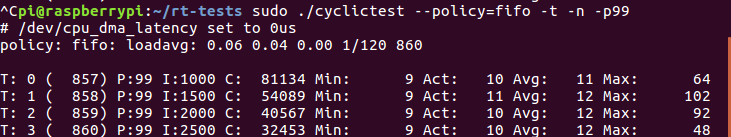
\includegraphics[width=16cm]{Voluntary-Fifo-WithoutHackbench.png}
\caption{SHED\_FIFO volontary}
\end{figure}
\begin{figure}[H]
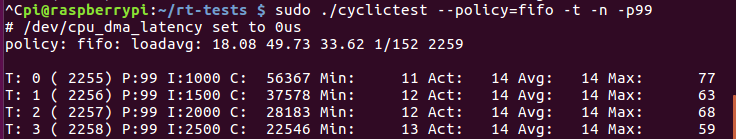
\includegraphics[width=16cm]{Preempt-Fifo-WithoutHackbench.png}
\caption{SHED\_FIFO preempt-rl}
\end{figure}
\subsubsection{SHED\_RR}
\begin{figure}[h]
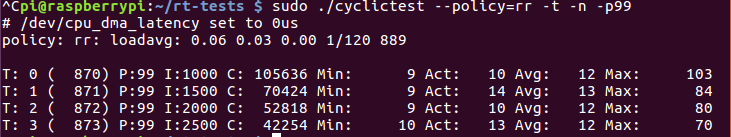
\includegraphics[width=16cm]{Voluntary-RR-WithoutHackbench.png}
\caption{SHED\_RR volontary}
\end{figure}
\begin{figure}[H]
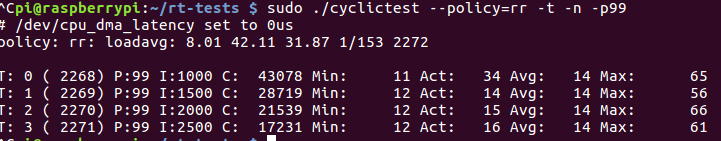
\includegraphics[width=16cm]{Preempt-RR-WithoutHackbench.png}
\caption{SHED\_RR preempt-rl}
\end{figure}
\subsubsection{Conclusion}
We observe that throughout all the different schedules have about similar avenged execution times with a slight advantage for the voluntary kernel. But, we there is a much higher maximum times for the voluntary kernel than the pre-emptive kernel, this is because the pre-emptive kernel was designed for consistency and to give a best worst case latency by minimizing the part of the kernel that can not be pre-empted.  This has negative effects on the advantage execution time that is worst than in the volontary kernel \footnote{to help improve the situation lazy pre-emption was introduced for SHED\_OTHER, see more \url{https://lwn.net/Articles/522144/}} as more overhead is necessary to ensure this determinism behaviour. This involves mechanisms such as priority inheritance to avoiding deadlocks or real-time throttling.

%Todo need shed other to conclude
\subsection{Cyclictest + Hackbench}
\subsubsection{Hackbench under SHED\_OTHER and priority 20}
\begin{figure}[H]
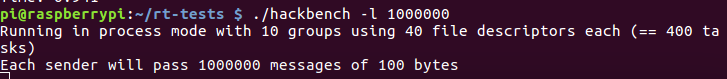
\includegraphics[width=16cm]{Volontary-other-Hackbench-p20.png}
\caption{Hackbench under SHED\_OTHER and priority 20}
\end{figure}
\subsubsection{Volontary}
\begin{figure}[H]
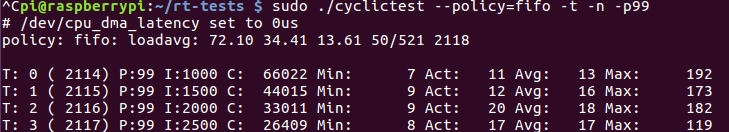
\includegraphics[width=16cm]{Volontary-Fifo-WithHackbench1.png}
\caption{Volontary fifo with hackbench}
\end{figure}
\begin{figure}[H]
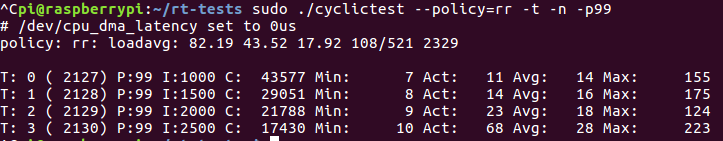
\includegraphics[width=16cm]{Volontary-Rr-WithHackbench1.png}
\caption{Volontary rr with hackbench}
\end{figure}
\subsubsection{Preempt-rt}
\begin{lstlisting}[language=bash,caption={Preempt fifo with hackbench}]
pi@raspberrypi:~/rt-tests$ sudo ./cyclictest --policy=fifo -t -n -p99
policy: fifo: loadavg: 130.65 51.20 18.86 85/551 1404           

T: 0 ( 1396) P:99 I:1000 C: 106248 Min:      7 Act:   26 Avg:   20 Max:      78
T: 1 ( 1397) P:99 I:1500 C:  70832 Min:      7 Act:   18 Avg:   20 Max:      73
T: 2 ( 1398) P:99 I:2000 C:  53124 Min:      7 Act:   24 Avg:   20 Max:      73
T: 3 ( 1399) P:99 I:2500 C:  42499 Min:      9 Act:   22 Avg:   21 Max:      74
\end{lstlisting}
\begin{lstlisting}[language=bash,caption={Preempt rr with hackbench}]
pi@raspberrypi:~/rt-tests$ sudo ./cyclictest --policy=rr -t -n -p99 
policy: rr: loadavg: 133.77 95.30 43.45 100/551 1454          

T: 0 ( 1450) P:99 I:1000 C:  70877 Min:      8 Act:   20 Avg:   20 Max:      91
T: 1 ( 1451) P:99 I:1500 C:  47251 Min:      8 Act:   20 Avg:   21 Max:      83
T: 2 ( 1452) P:99 I:2000 C:  35438 Min:      9 Act:   23 Avg:   21 Max:      69
T: 3 ( 1453) P:99 I:2500 C:  28350 Min:      9 Act:   21 Avg:   21 Max:      92
\end{lstlisting}

\subsubsection{Hackbench under RT scheduling policies and priority 49}
\subsubsection{SHED\_FIFO}
\begin{figure}[H]
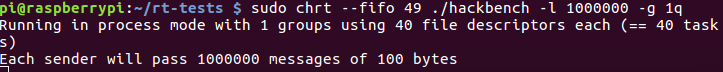
\includegraphics[width=16cm]{Hackbench2.png}
\caption{Hackbench with shed\_fifo and priority 49}
\end{figure}
\begin{figure}[H]
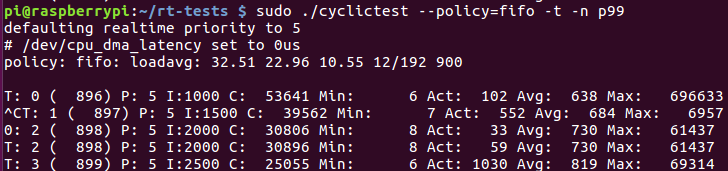
\includegraphics[width=16cm]{Preempt-Fifo-WithHackbench2.png}
\caption{Volontary with fifo}
\end{figure}
\begin{figure}[H]
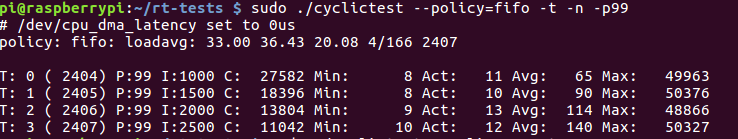
\includegraphics[width=16cm]{Volontary-Fifo-WithHackbench2.png}
\caption{Preempt-rt with fifo}
\end{figure}
\subsubsection{SHED\_RR}
\begin{lstlisting}[language=bash,caption={Hackbench with shed\_rr and priority 49}]
pi@raspberrypi:~/rt-tests$ \textsc{sudo chrt --rr 49 ./hackbench -l 1000000 -g 1q                     }
Each sender will pass 1000000 messages of 100 bytes
\end{lstlisting}
\begin{figure}[H]
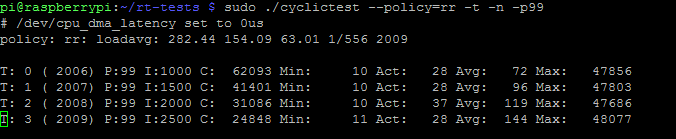
\includegraphics[width=16cm]{Preempt-RR-WithHackbench.png}
\caption{Preempt-rt with fifo}
\end{figure}
\begin{lstlisting}[language=bash,caption={Volontary kernel}]
sudo ./cyclictest --policy=rr -t -n -p99
policy: rr: loadavg: 29.39 27.96 14.37 32/161 848          

T: 0 (  832) P:99 I:1000 C: 338191 Min:      8 Act:   18 Avg:   67 Max:   49660
T: 1 (  833) P:99 I:1500 C: 225480 Min:      8 Act:   54 Avg:   96 Max:   49563
T: 2 (  834) P:99 I:2000 C: 169312 Min:      8 Act:   18 Avg:  118 Max:   49511
T: 3 (  835) P:99 I:2500 C: 135316 Min:      9 Act:   19 Avg:  144 Max:   47964
\end{lstlisting}
\subsubsection{Consclusion}
With hackbench we are introducing significant stress on our systems and are truly revealing the core difference between the voluntary and the full preemptable kernel : consistency. Avenged times are grouped more closely and although minimum times are vagly similar the interval between minimum and maximum times are vastly different in favour of the pre-emptable kernel.
This is particularly apparent when hackbench is given a priority of 49 and using fifo. As our task have a higher priority we are pre-empting the hackbench tasks and running the cyclictest instead in the case of the preepmt-rt kernel. On the other hand the voluntary kernel is unable to perform they types of pre-emptions: the kernel has no way of interrupting these running routines \textit{eg : a systemcall}. The problem now is that hackbench's principal revolves around systemcalls: the voluntary kernel's tasks will not be able to preempt\footnote{It's dead jim.}.\\
Hackbench code : \\
\url{https://github.com/linux-test-project/ltp/blob/master/testcases/kernel/sched/cfs-scheduler/hackbench.c}
\begin{figure}[H]

\begin{lstlisting}
	for (i = 0; i < loops; i++) {
		for (j = 0; j < ctx->num_fds; j++) {
			int ret, done = 0;

again:
			ret =
			    write(ctx->out_fds[j], data + done,
				  sizeof(data) - done);
			if (ret < 0)
				barf("SENDER: write");
			done += ret;
			if (done < sizeof(data))
				goto again;
		}
}

\end{lstlisting}
\caption{Hackbench : Sender code}
\end{figure}
\begin{figure}[H]
\begin{lstlisting}
	/* Receive them all */
	for (i = 0; i < ctx->num_packets; i++) {
		char data[DATASIZE];
		int ret, done = 0;

again:
		ret = read(ctx->in_fds[0], data + done, DATASIZE - done);
		if (ret < 0)
			barf("SERVER: read");
		done += ret;
		if (done < DATASIZE)
			goto again;
	}
\end{lstlisting}
\caption{Hackbench : reciver code}
\end{figure}
\section{ADA concurrent programs}
\subsection{Program 1}
\paragraph{code}
\begin{figure}[H]
\begin{center}
\verbatiminput{main.adb}
\caption{Program 1}
\end{center}

\end{figure}

\paragraph{Observations}
The A,B,C,D are printed in order throughout the execution with there not being any apparent modification of that ordered sequence.
\subsection{Program 2}
\paragraph{code}
\begin{figure}[H]
\begin{center}
\verbatiminput{main2.adb}
\caption{Program 2}
\end{center}
\end{figure}

\paragraph{Observations}
In this test we can observe that even though both treads are configure to sleep for the same 100ms time interval they eventually end up off sync. We can attribute this to the difference between the way time is treated in the \emph{delay} and \emph{delay until}.
\\
%diffrence
\subparagraph{delay}
This main difference is that \emph{delay} uses an \textit{approximate relative time delay}. It measured the time from a specific reference point . If this reference point is displaced in time by the process being pre-empted for example this  introduces a delay of \emph{at least} the amount of time specified,not the exact specified task. This introduced local drift (delay) can be cumulated resulting in this de-synchronization.
If we wanted delay to wait for an absolute time then the task would have to run uninterrupted by any other task which is not the case here.
\subparagraph{delay until}
This statement schedules for an absolute wake-up task, this works by making the task not schedule until the interval time has elapsed. Her again there is no guaranty on the actual time the task will be executed if for example the resource required to handle that task is not available ( used by a higher priority task , ect ... ) the task will still eventually stall. Yet, as there is no resource sharing in this case we can amuse that the task will be handled immediately\footnote{With very little latency} after it is marked as ready.
\end{document}